
\documentclass{Beamer}

%

			% Packages Files
%----------------------------------%

%	% Page Setttings
%\usepackage[top = 1in, bottom = 1in, left = 1in, right = 1in]{geometry}
%
%\parindent=0cm % to prevent the spacing in new paragraph or new line
%
%\usepackage{fancyhdr} % needded for header and footer 

%-----------------------------------------------------------------%

\usepackage{amsmath} % needed for referencing thequation
\usepackage{amsfonts} % for maths symbols
\usepackage{graphicx}
\usepackage[export]{adjustbox}
\usepackage{caption}
\usepackage{refstyle} % to reference a captioned figure


% To make hyperlinks

\usepackage[
	colorlinks=true
	,breaklinks
	]{hyperref} % needed for creating hyperlinks in the document, the option colorlinks=true gets rid of the awful boxes, breaklinks breaks lonkg links (list of figures),
	
\usepackage{xcolor}
\definecolor{c1}{rgb}{0,0,1} % blue
\definecolor{c2}{rgb}{0,0.3,0.9} % light blue
\definecolor{c3}{rgb}{0.3,0,0.9} % red blue
\hypersetup{
    linkcolor={c1}, % internal links
    citecolor={c2}, % citations
    urlcolor={c3} % external links/urls
}

	% For Code Writing
	
\usepackage{listings}

\usepackage{color}

\definecolor{mygreen}{rgb}{0 0.6 0}

\lstset{
% Set automatic Line breaking, in case we have long lines don't
% fit inside the frame or the page.
breaklines = true,
commentstyle = \color{mygreen},
breakatwhitespace = true,% don't show white space character
%numbers = left, % put line number in the code
title = \lstname
}

% ------------- For Writing Equations inisde a table and centering them ------------

\usepackage{array}

% Vertical Alignment inside the cells of the table
\newcolumntype{M}[1]{>{\centering\arraybackslash}m{#1}}

% Horizontal Alignment inside the cells of the table
\newcolumntype{P}[1]{>{\centering\arraybackslash}p{#1}}




% Macros File

% Macros Example
\def\labelaxes{Remember to include some suitable labeling for the axes and the units used in measurements.}

% 2nd way for defnining macros: the new command
% 1st parameter: name of the new command
% 2nd paramter: how many inputs this command needs, in this case only 1
% 3rd parameter: what this new command named \tbi do

\newcommand{\tbi}[1]{\textbf{\textit{#1}}}

% Command for Picture without a label

\newcommand{\pic}[3]{\begin{figure}[h]
\centering
\includegraphics[width = 0.7\textwidth, frame]{#1}
\caption{#2}
\end{figure}}






%\usepackage{natbib}

\setbeamertemplate{bibliography item}{\insertbiblabel}

%\usetheme{Warsaw}

%% Foot Options
\usenavigationsymbolstemplate{} % deafult controls off
%\setbeamertemplate{page number in head/foot}[totalframenumber] 

\setbeamertemplate{footline}[frame number]
% display slide number/ total number of slides

% To split the frame into 2 or more columns
\usepackage{multicol}

%% Fonts
\usefonttheme{professionalfonts} % changes fonts

% ----------------- Tikz Package --------------

\usepackage{tikz}

\usetikzlibrary{shapes,shadows,arrows}

% for displaying number of figures in the caption
\usepackage{graphicx,caption}

\usepackage{xcolor}

\DeclareMathOperator*{\argmax}{argmax}

% for code writing
\usepackage{listings}

\title[DEEPEMBED]{Stage Memo and Presentations}
%\subtitle{Subtitle Here}
\author{Done by: Ranim Tom}


%In case I don't want the date to appear in the slides
\date[]




%*******************************************************


\begin{document}

%\metroset{block=fill}

\begin{frame}
\titlepage
\end{frame}


% A content slide
% [t] for displaying the content at the 
%top of the slide.


\begin{frame}{Table of Contents}
%\tableofcontents
%This command if we want to display only sections
%without subsections
\tableofcontents[hideallsubsections]
\end{frame}


\section{Learning audio representations
with self-supervision}





\begin{frame}[t]{Learning audio representations with self-supervision \cite{Audio2Vec}}

Goal of this paper:

\begin{itemize}

\item Apply self supervision to learn general purpose audio representations using 2 self supervised task: 

	\begin{itemize}
	\item Audio2Vec: aims to reconstruct a spectrogram slice from past and future slice  
	
	\item TemporalGap: estimates the distance between two short audio segments extracted at random from the same audio clip
	\end{itemize}


\end{itemize}


\end{frame}


\subsection{Introduction}
\begin{frame}[t,allowframebreaks]{Introduction}


\begin{itemize}

\item Disadvantage of supervised learning altough the major advancement it has done:


\begin{enumerate}
\item requires collecting
large annotated datasets specific to each task to be solved

\item separate models are typically trained for each task,
making it difficult to reuse computational resources when
multiple such models are deployed on a mobile device
\end{enumerate}

\item Solution to this: using unsuperivsed learning approach, specifically self supervised where:

	\begin{itemize}
	\item formulates an \textcolor{red}{auxiliary task} based on the available \textcolor{red}{unlabelled data}
	
	\item the model will learn some general purpose representations in a lower dimensional embedding space while solving this auxiliary task 
	
	\item As a result, the embedding
\textcolor{red}{encoder}, e.g., the portion of the model architecture mapping the input data to the embedding space, can be \textcolor{red}{reused as a feature extractor for different downstream tasks}.
	\end{itemize}

\item One of the earliest successes of self-supervised learning
was obtained in the context of language models is Word2Vec, where it comes in 2 format:
	\begin{enumerate}
	\item Continuous bag-of-words (CBoW): the model predicts the current word based on the context of surrounding words
	
	\item skip-gram: predicts surrounding words given the current word
	\end{enumerate}

\end{itemize}


\end{frame}



\subsection{Self Supervised Part}
\begin{frame}[t]{Self Supervised Part: Auxiliary Task Proposed}


\begin{figure}[h]
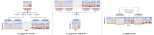
\includegraphics[scale=0.60]{Figures/Audio2Vec_Diagram.pdf}
\caption{Overview of the proposed self-supervised learning tasks  \cite{Audio2Vec}}
\end{figure}

\begin{itemize}
\item In CBoW formulation the auxiliary task consists of reconstructing a temporal slice of pre-determined duration from a number of past and future slices.
\end{itemize}

\end{frame}

\subsection{Description of Audio2Vec: CBoW Formulation}
\begin{frame}[t,allowframebreaks]{Description of Audio2Vec: CBoW Formulation} 

\begin{itemize}

\item Let $x$ be an audio clip of $n$ samples, $x \, = \, [\, x_1 \, , \, x_2 \, , \,  \cdots \, , x_n \,]$

\item $x \, \mapsto \, X \in \mathbb{R}^{T \, \times \, F}$, where $\begin{cases}

X: \text{Sepctrogram of } x \\
T: \text{number of temporal frames} \\
F: \text{frequency bins}
\end{cases}$.

\item The authors randomly pick a slice of $X$ denoted by $X_i \, \in \,\mathbb{R}^{N \, \times \, F}$ such that $N \, < \, T$.

\item  Let's say that $X_i \, = \, X_{(0)}$. The next step is to pick some other slices of the same audio clip $x$, before and after the slice $X_{(0)}$.

	\begin{itemize}
	\item More specifically, we have \textcolor{red}{past slices} denoted by $\{ X_{(-P)} \, , \, \cdots \, , \, X_{(-1)} \}$ and \textcolor{red}{future slices} denoted by $\{ X_{(1)} \, , \, \cdots \, ,\, X_{(P)} \}$
	\end{itemize}

\item Each slice from $ X_{(-P)} \, \rightarrow \, X_{(P)}$ will be processed by the same encoder denoted by \textit{Enc}, and as an output we obtain an \textcolor{red}{embedding vector} $z_{(p)}$.

	\begin{itemize}
	\item $Enc(X_{P}) \, = \, z_{(p)}$
	\end{itemize}

\item Then a vector $\bar{z}_{(0)}$ is obtained by concatenating all the embedding vector and inputted to a convolutional decoder to obtain a reconstruction of the slice $X_{(0)}$

	\begin{itemize}
	\item Concatenating $\bar{z}_{(0)} \, = \, \left[ \, z_{(-P)} \, , \, \cdots \, , \, z_{(-1)} \, , \, z_{(1)} \, , \, \cdots \, ,\, z_{(P)}   \,\right]$
	
	\item Decoder: $ \hat{X}_{(0)} \, = \, Dec(\bar{z}_{(0)})$
	\end{itemize}

\item Objective Function: the overall encoder-decoder is trained using MSE: $\parallel X_{(0)} \, - \,  \hat{X}_{(0)} \parallel$

\end{itemize}

\end{frame}

\subsection{Encoder-Decoder Architecture}
\begin{frame}[t,allowframebreaks]{Description of Audio2Vec: Encoder-Decoder Architecture}

\begin{itemize}

\item Concerning the decoder part:

	\begin{itemize}
	\item Reversing the order of the convolutional layer in the encoder part
	
	\item Replacing max-pooling with nearest-neighbor upsampling
	\end{itemize}


\item Raw Audio Signal Processing:
	
	\begin{itemize}
	\item sampling frequency = 16 kHz
	
	\item Window size of 25 ms and hop length of 10 ms to compute the STFT 
	
	\item Computing  mel spectrogram by using 64 frequency bins in the range of 60-7800 Hz 	 	
	
	
	\end{itemize}


\item Encoder Architecture: 6 layers all having $3 \, \times \, 3$ filter, with channel numbers respectively equal to [64, 128, 256, 256, 512, 512]

\end{itemize} 

\end{frame}





\begin{frame}[t]{Description of Audio2Vec: Adapting to SpecCense}

\begin{figure}[h]
\includegraphics[scale=0.35]{Figures/Relation_Audio2Vec_SpecCense.pdf}
\caption{Relation to SpecCense Data}
\end{figure}

\end{frame}



\begin{frame}[t]{Description of Audio2Vec: Adapting to SpecCense}


\begin{figure}[h]
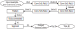
\includegraphics[scale=0.45]{Figures/Felix_Archi}
\caption{Adapting to Felix Architecture}
\end{figure}

\end{frame}


\section{Preparing the SpecCense Dataset}

\begin{frame}[t]{Step 1: Slicing the frames}

\begin{figure}[h]
\centering
\includegraphics[scale=0.34]{Figures/Data_Preparation_Step_1_Slicing.pdf}
\caption{Frame Slicing}
\end{figure}

\end{frame}



\begin{frame}[t]{Step 2: Stacking into matrix $X$}

\begin{columns}[onlytextwidth]



\column{0.4\textwidth}

\begin{figure}[h]
\centering
\includegraphics[scale=0.32]{Figures/Data_Preparation_Step_2_Stacking_into_matrix.png}
\end{figure}


\column{0.4\textwidth}

$ \begin{bmatrix}

\vdots &  \cdots & \vdots \\
\vdots &  \cdots & \vdots \\

29 \, \times \, \text{w} &  
\cdots & 29 \, \times \, \text{w} &\\

\vdots &  \cdots & \vdots \\
\vdots &  \cdots & \vdots \\
\end{bmatrix}$




\end{columns}

\begin{itemize}

\item The matrix $X$ will contain the \textcolor{red}{total samples}, in which we will split them into train, validation and test set.

\item shape of $X$:
$
\begin{cases}
\text{number of rows: } 29 \, \times \, \text{width} \\
\text{number of columns: } \text{iteration per csv file} \\
\text{iteration per csv file} = \text{math.floor(number of frames / width)}

\end{cases}$

\end{itemize}




\end{frame}



\begin{frame}[t]{Time Continuity}

\begin{figure}[h]
\centering
\includegraphics[scale=0.32]{Figures/Time_Continuity.pdf}
\end{figure}

\begin{itemize}

\item In case there is a discontinuity, do I reject all the slice (the training sample)? 

\end{itemize}


\end{frame}


\begin{frame}[t]{Pretext Task}

\begin{figure}[h]
\centering
\includegraphics[scale=0.35]{Figures/Pretext_Task.pdf}
\end{figure}




\end{frame}


%------------ References ------------------------
\section{References}


\begin{frame}[allowframebreaks]
\frametitle{References}

\bibliographystyle{IEEEtran}
\frametitle{References}
\bibliography{literature/Deep_Learning_Papers_References}

\end{frame}

%\bibliographystyle{IEEEtran}
%\frametitle{References}
%\bibliography{literature/LIDAR_Remote_Sensing}



%------------- End of References -------------------


\end{document}